\documentclass[border=0pt,varwidth=14cm,convert={outext=.jpg,density=300}]{standalone}%
\usepackage{amsmath,graphicx,array,xcolor}%
\graphicspath{{../figures/}}
\begin{document}\pagecolor{white}%
\newcolumntype{C}{>{\centering\arraybackslash} m{6cm} }
\begin{figure}[h!]\centering
	\begin{tabular}{m{1cm}CC}
		& $\log O^{7+}/O^{6+}$ & $V_{sw}$ \\ \\
		CHW & 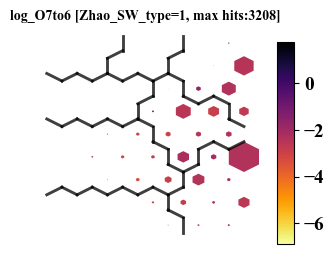
\includegraphics[width=6cm]{Amaya/SWtype-Zhao_SW_type-1-log_O7to6} &
		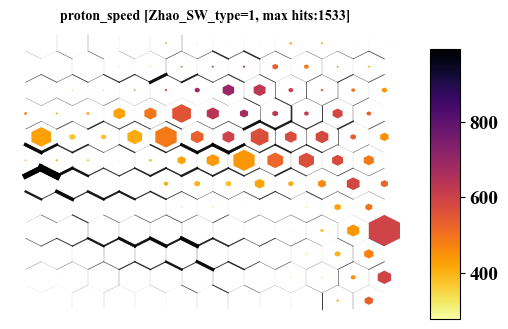
\includegraphics[width=6cm]{Amaya/SWtype-Zhao_SW_type-1-proton_speed}\hfill	\\
		ICME & 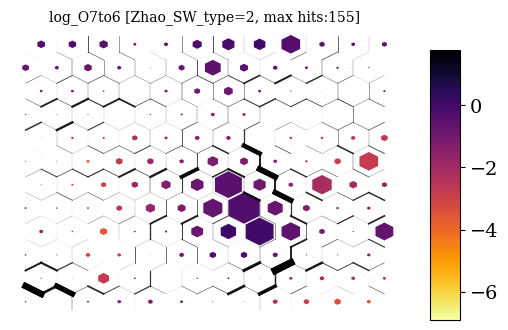
\includegraphics[width=6cm]{Amaya/SWtype-Zhao_SW_type-2-log_O7to6} &
		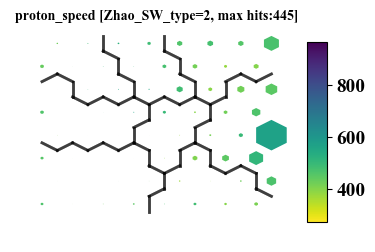
\includegraphics[width=6cm]{Amaya/SWtype-Zhao_SW_type-2-proton_speed}\hfill	\\
		NCHW & 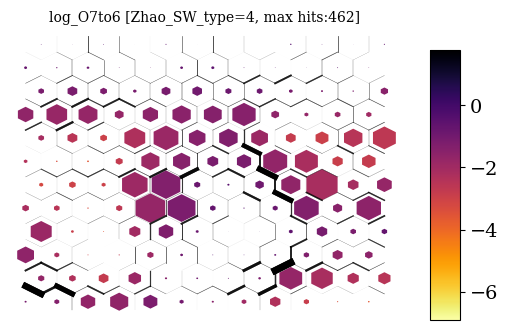
\includegraphics[width=6cm]{Amaya/SWtype-Zhao_SW_type-4-log_O7to6} &
		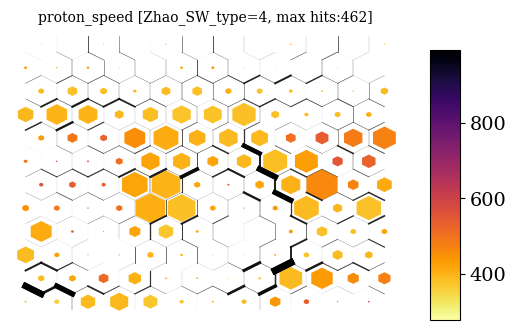
\includegraphics[width=6cm]{Amaya/SWtype-Zhao_SW_type-4-proton_speed}\hfill \\
	\end{tabular}
\end{figure}
\end{document}%